\documentclass[10pt,french]{book}
\input preambule_2013

\newcounter{exoc}
\newenvironment{exoc}[1]{%
  \refstepcounter{exoc}\textbf{Exercice \theexoc} :\hfill {\textbf{#1}}\par
  \medskip}%
{\medskip}

\begin{document}

\pieddepage{}{}{}

\begin{center}
\begin{tabularx}{\textwidth}{|>\centering m{2.5cm}|>\centering X|>{\centering\arraybackslash} m{2.5cm}|}
	\hline
		1\iere \bsc{e.e.a.c.} & Lundi 18 novembre \np{2013} & \textbf{Trigonométrie} \\
	\hline
		\multicolumn{3}{|c|}{\bsc{Contrôle de mathématiques}} \\
	\hline
        \multicolumn{1}{|r}{\bsc{Nom}:} & \multicolumn{2}{l|}{} \\
		\multicolumn{1}{|r}{Prénom:} & \multicolumn{2}{l|}{} \\
	\hline
        \multicolumn{3}{|l|}{\bfseries Note et observations :} \\[1cm]
    \hline
\end{tabularx}\bigskip

{\itshape
La qualité et la précision de la rédaction seront prises en compte dans l'appréciation des copies.\par
Le barème est indicatif.}
\end{center}

\begin{exoc}{2 pts}
    Donner la mesure principale de l'angle dont une mesure est $a = \dfrac{98\pi}{5}$.
\end{exoc}

\begin{exoc}{5 pts}
    On a représenté sur le repère \OIJ ci-dessous le cercle trigonométrique $\calig U$ et un point $M \in \calig U$ tel que $\widehat{IOM} = \rad\alpha$.
    
    \begin{minipage}{0.55\linewidth}
        \begin{enumerate}
        	\item Placer \textbf{de façon précise} sur $\calig U$ les points $A$, $B$, $C$ et $D$ repérés respectivement par les réels :
                \[-\dfrac{5\pi}{6} \qq \dfrac{\pi}{3} \qq -\dfrac{\pi}{3} \qetq \dfrac{3\pi}{4}.\]
        	\item Sur votre copie, écrire les coordonnées \textbf{exactes} des quatre points $A$, $B$, $C$ et $D$.
            \item Placer sur $\calig U$ le point $N$ tel que $\widehat{ION} = -\alpha$.
            \item Placer sur $\calig U$ le point $P$ tel que $\widehat{IOP} = \pi -\alpha$.
        \end{enumerate}
    \end{minipage}\hfill
    \begin{minipage}{0.45\linewidth}
        \begin{center}
            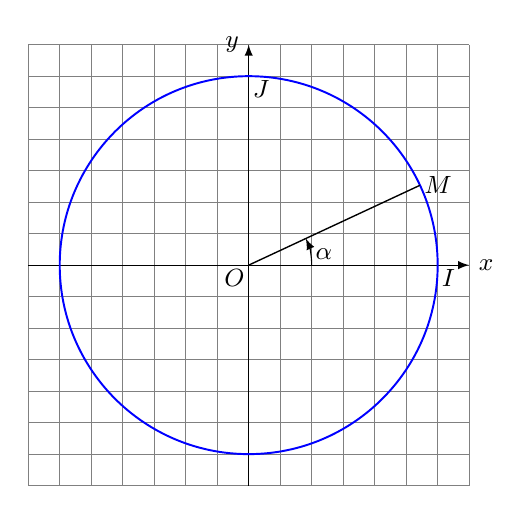
\begin{tikzpicture}[>=latex,scale=0.4]
                \draw[help lines] (-7,-7) grid (7,7);
                \draw[->,line width=0.4pt] (-7,0) -- (7,0) node[right] {\small $x$};
                \draw[->,line width=0.4pt] (0,-7) -- (0,7) node[left] {\small $y$};
                \draw[line width=0.7pt,blue] (0,0) circle (6);
                \draw (0,0) node[below left = -2pt] {\small $O$};
                \draw (6,0) node[below right = -2pt] {\small $I$};
                \draw (0,6) node[below right = -2pt] {\small $J$};
                \draw[line width = 0.5pt] (0,0) -- (25:6) node[right=-2pt] {\small $M$};
                \draw[->] (2,0) arc (0:25:2) node[below right] {\small $\alpha$};
            \end{tikzpicture}
        \end{center}
    \end{minipage}
\end{exoc}

\begin{exoc}{4 pts}
Résoudre dans $\R$ les équations suivantes :
\begin{enumerate}
	\item $\sin(t) = \sin \left(\dfrac{\pi}{3}\right)$.
	\item $\cos(t) - \dfrac{\sqrt{3}}{2} = 0$.
\end{enumerate}
\end{exoc}


\begin{exoc}{4 pts}
 \'Ecrire en fonction de $\cos(x)$ ou de $\sin(x)$ les expressions suivantes :
 \[A = \cos(-x) \qq B = \cos(\pi - x) \qq C = \sin(-x) \qq D = \sin(\pi - x).\]
 \[E = 3\cos(\pi - x) + 2\cos(2\pi + x) - 3\cos(-x) \qetq F = 2\sin(x) + 2\sin(\pi - x) - 4\sin(-x).\]
\end{exoc}

\begin{exoc}{5 pts}
On rappelle la formule suivante : $\cos^2(x) + \sin^2(x) = 1.$\par
On donne $\beta = \dfrac{\pi}{8}$ et $\cos (\beta)= \dfrac{\sqrt{2 + \sqrt 2}}{2}$.	
\begin{enumerate}
	\item Calculer $\cos^2(\beta)$.
    \item En déduire la valeur de $\sin(\beta)$ \textbf{en justifiant précisément le signe du résultat}.
    \item \textbf{En détaillant précisément les étapes,} en déduire la valeur de $\sin\left(-\dfrac{7\pi}{8}\right).$
\end{enumerate}
\end{exoc}

\end{document} 